\documentclass[crop,tikz]{standalone}

\usepackage{tikz}
\tikzset{mynode/.style={inner sep=2pt,fill,outer sep=0,circle}}

\begin{document}

\begin{center}
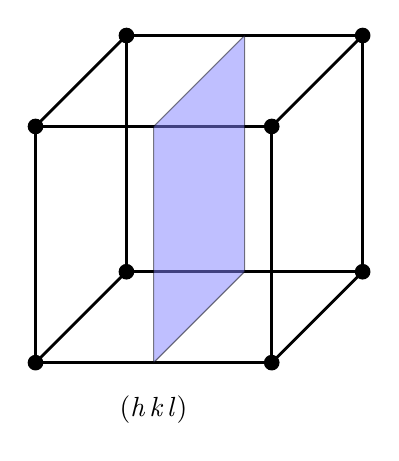
\begin{tikzpicture}[scale=3,line width=1pt]
 \coordinate (1) at (0,0,0);
 \coordinate (2) at (0,1,0);
 \coordinate (3) at (1,1,0);
 \coordinate (4) at (1,0,0);
 \coordinate (5) at (0,0,1);
 \coordinate (6) at (0,1,1);
 \coordinate (7) at (1,1,1);
 \coordinate (8) at (1,0,1);
 \foreach \x in {1,2,...,8}{
     \node[mynode] at (\x) {};
 }
 \draw (1) -- (2) -- (3) -- (4) -- cycle;
 \draw (5) -- (6) -- (7) -- (8) -- cycle;
 \draw (1) -- (5)  (2) -- (6) (3) -- (7) (4) -- (8);
 \draw[thin,fill=blue!50,opacity=0.5] (0.5,0,0) -- (0.5,0,1) -- (0.5,1,1) -- (0.5,1,0) --cycle;
 \node at (0.5,-0.2,1) {(\textit{h\,k\,l})};
\end{tikzpicture}
\hspace{1cm}
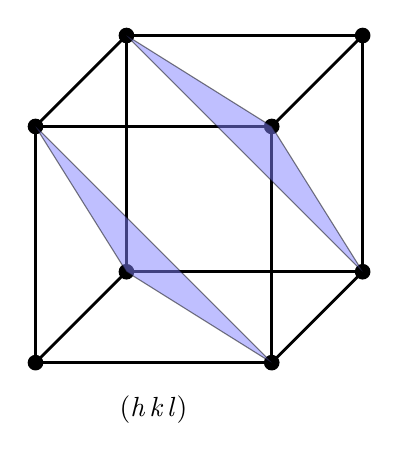
\begin{tikzpicture}[scale=3,line width=1pt]
 \coordinate (1) at (0,0,0);
 \coordinate (2) at (0,1,0);
 \coordinate (3) at (1,1,0);
 \coordinate (4) at (1,0,0);
 \coordinate (5) at (0,0,1);
 \coordinate (6) at (0,1,1);
 \coordinate (7) at (1,1,1);
 \coordinate (8) at (1,0,1);
 \foreach \x in {1,2,...,8}{
     \node[mynode] at (\x) {};
 }
 \draw (1) -- (2) -- (3) -- (4) -- cycle;
 \draw (5) -- (6) -- (7) -- (8) -- cycle;
 \draw (1) -- (5)  (2) -- (6) (3) -- (7) (4) -- (8);
 \draw[thin,fill=blue!50,opacity=0.5] (1) -- (8) -- (6) --cycle;
 \draw[thin,fill=blue!50,opacity=0.5] (2) -- (4) -- (7) --cycle;
 \node at (0.5,-0.2,1) {(\textit{h\,k\,l})};
\end{tikzpicture}

\end{center}

\end{document}